\chapter{Finální podoba vestavěného systému}
    \label{sec:fotky}

    \begin{figure*}[h]
        \centering
        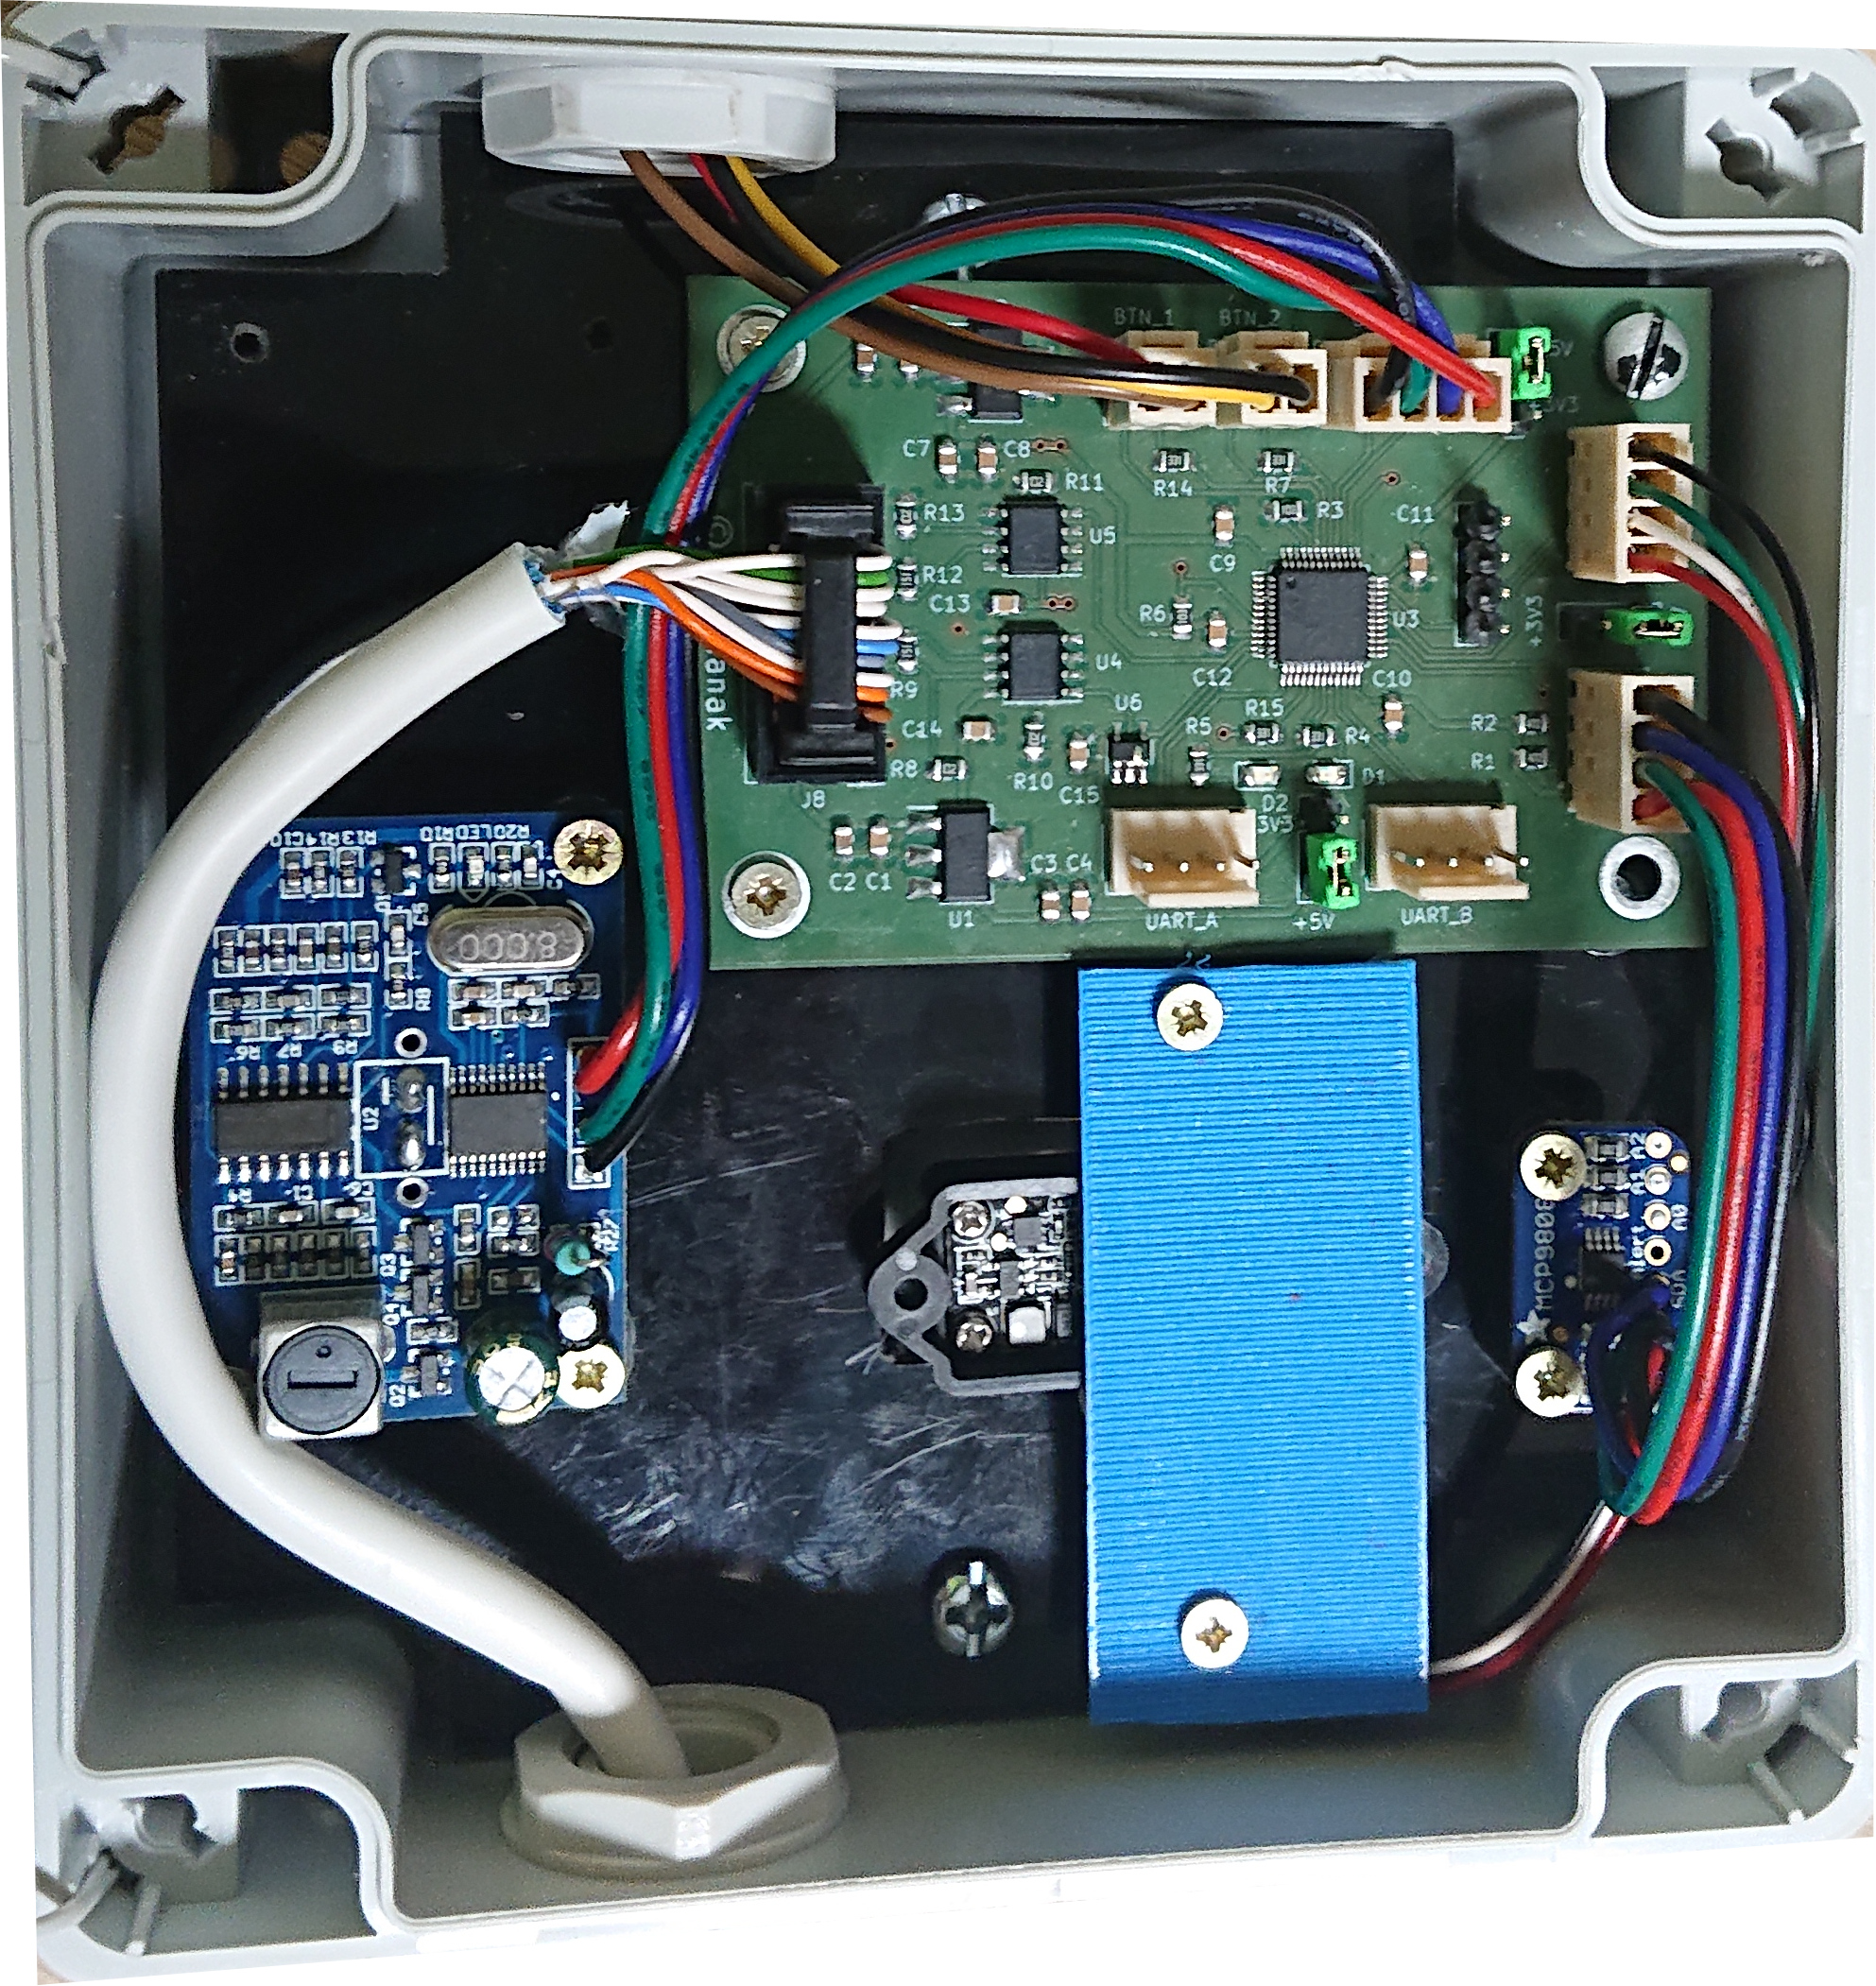
\includegraphics[width=0.6\linewidth]{obrazky-figures/done_01.JPG}
        \caption{Pohled na otevřenou krabici reprezentující řídicí část vestavěného systému.}
    \end{figure*}

    \begin{figure*}[h]
        \centering
        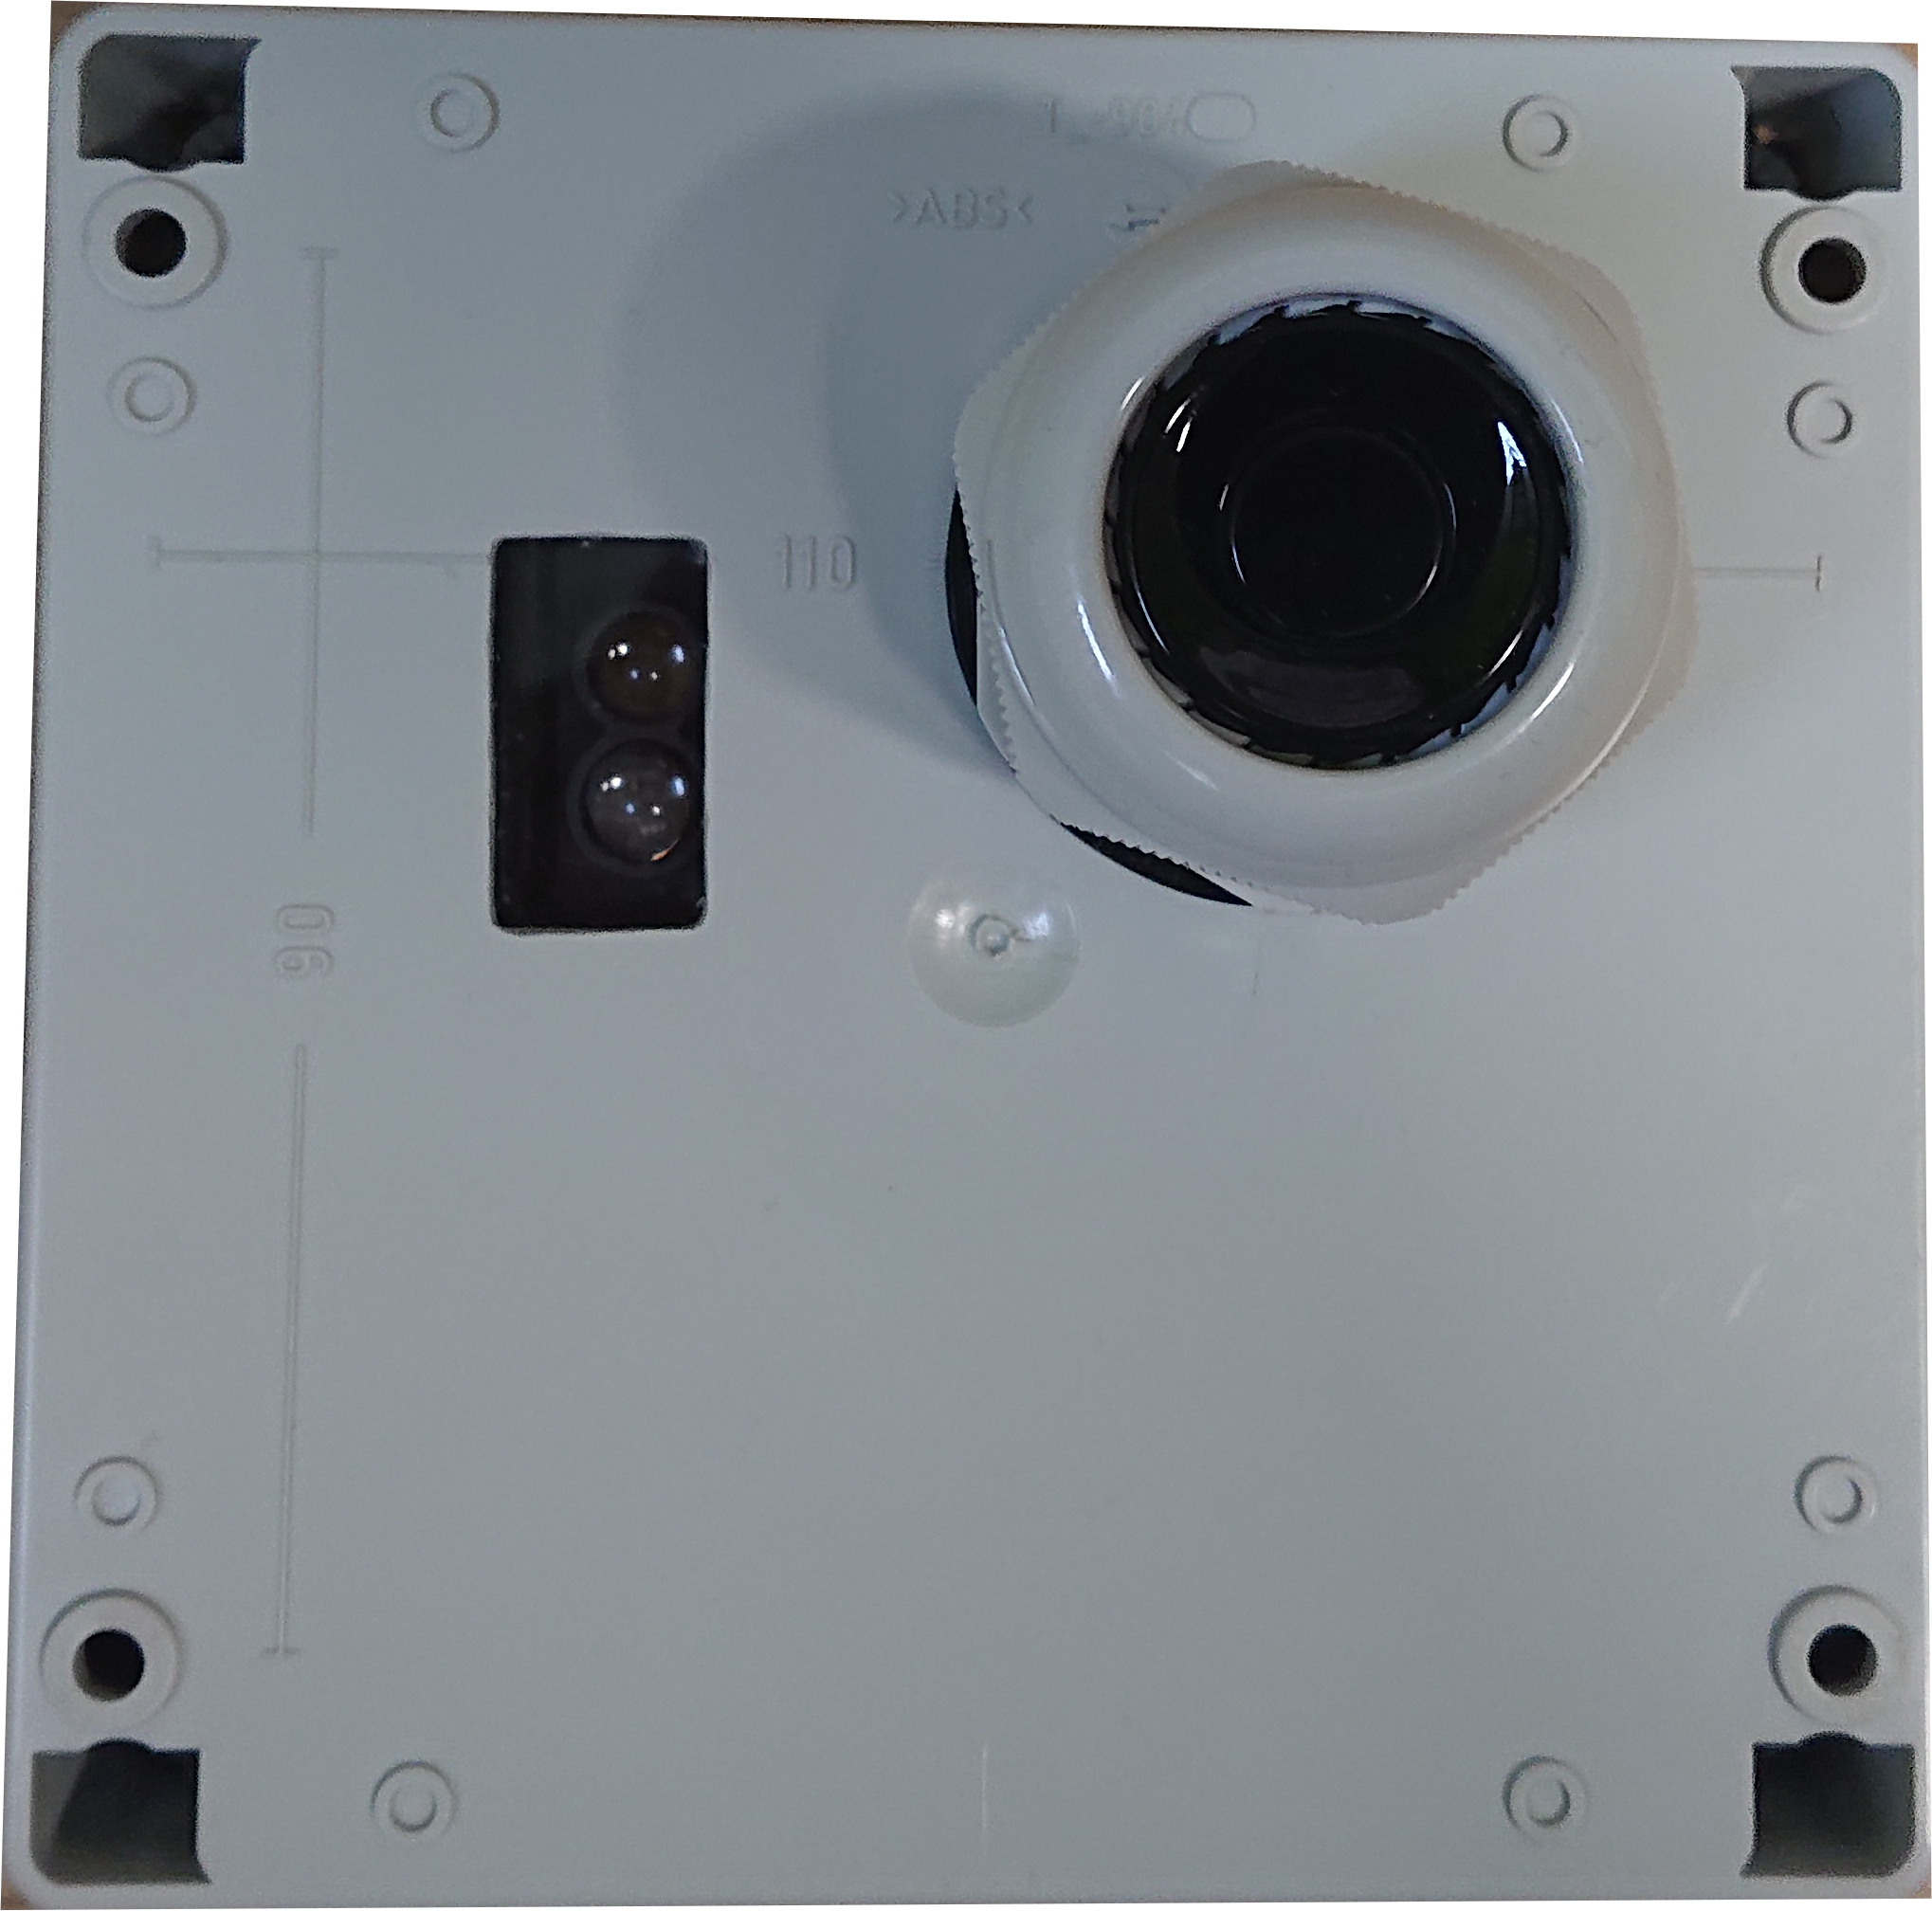
\includegraphics[width=0.6\linewidth]{obrazky-figures/done_03.JPG}
        \caption{Pohled na spodní část krabice reprezentující řídicí část vestavěného systému.}
    \end{figure*}

    \begin{figure*}[h]
        \centering
        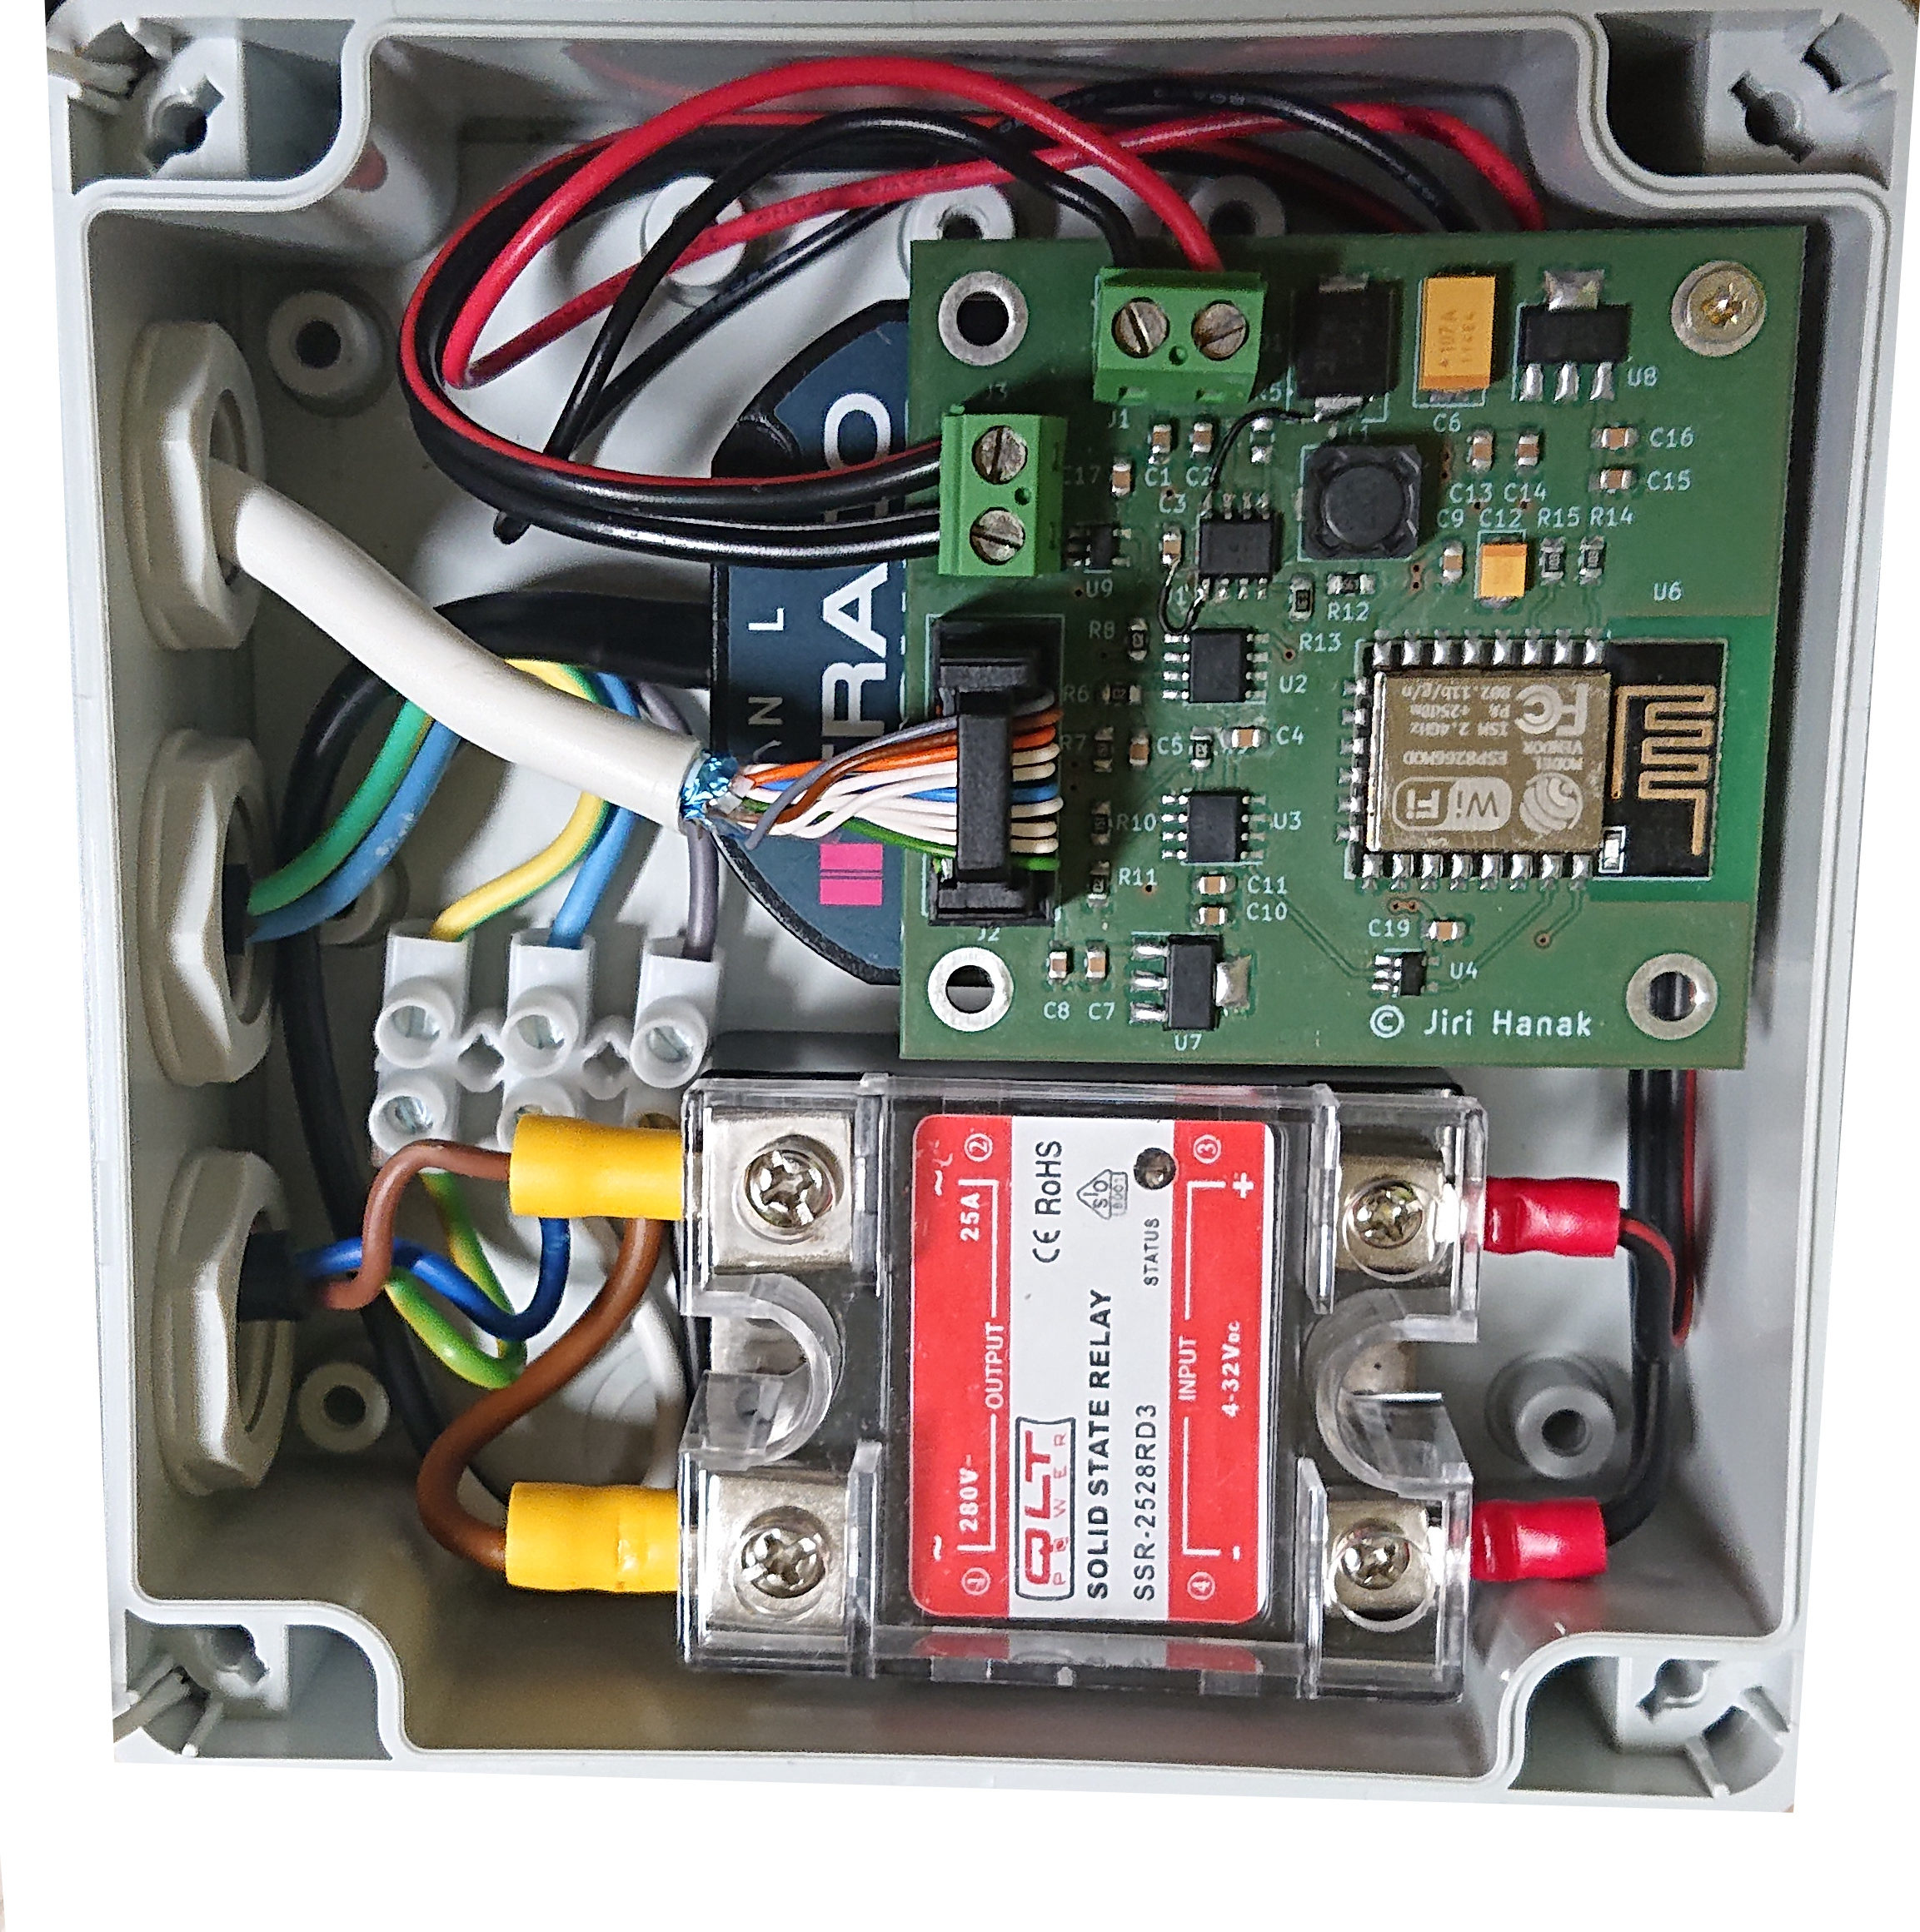
\includegraphics[width=0.6\linewidth]{obrazky-figures/done_02.JPG}
        \caption{Pohled na otevřenou krabici reprezentující podpůrnou část vestavěného systému.}
    \end{figure*}
\chapter{Výsledky testovacího měření TFmini a JSN-SR04T-2.0}
	\label{sec:values}
	\begin{table*}[h]\centering
        \begin{tabular}{@{}cccccccc@{}}
            \toprule
            \multirow{2}{*}{\textbf{Reference}} & \multicolumn{3}{c}{\textbf{TFmini}} && \multicolumn{3}{c}{\textbf{JSN-SR04T-2.0}}\\ 
            \cmidrule{2-4}\cmidrule{6-8}
            	& \textbf{Podlaha}    & \textbf{Voda}      & \textbf{Pěna}&& \textbf{Podlaha}    & \textbf{Voda}      & \textbf{Pěna}\\
            \midrule
            400		& 372	& 988	& 470	&& 398	& 353	& 357	\\ 
            500		& 486	& 1040	& 589	&& 506	& 448	& 452	\\ 
            600		& 590	& 1087	& 673	&& 601	& 558	& 558	\\ 
            700		& 680	& 1142	& 744	&& 691	& 644	& 665	\\ 
            800		& 782	& 1155	& 816	&& 795	& 750	& 756	\\ 
            900		& 872	& 1169	& 905	&& 896	& 853	& 853	\\ 
            1000	& 995	& 1212	& 1009	&& 1002	& 941	& 982	\\ 
            1100	& 1092	& 1240	& 1087	&& 1096	& 1047	& 1073	\\
            1200	& 1185	& 1255	& 1182	&& 1198	& 1183	& 1157	\\ 
            1300	& 1280	& 1321	& 1275	&& 1301	& 1247	& 1252	\\ 
            1400	& 1381	& 1408	& 1379	&& 1394	& 1355	& 1370	\\ 
            1500	& 1486	& 1511	& 1462	&& 1487	& 1459	& 1510	\\ 
            1600	& 1584	& 1631	& 1547	&& 1590	& 1592	& 1558	\\ 
            1700	& 1672	& 1718	& 1657	&& 1693	& 1655	& 1663	\\ 
            1800	& 1786	& 1790	& 1750	&& 1792	& 1741	& 1754	\\ 
            1900	& 1875	& 1899	& 1878	&& 1900	& 1853	& 1853	\\ 
            2000	& 1995	& 1998	& 1953	&& 1989	& 1976	& 1948	\\ 
            \bottomrule
        \end{tabular}
        \caption{V~tabulce jsou uvedeny změřené hodnoty optickým snímačem \io{TFmini} a ultrazvukovým snímačem \io{JSN-SR04T-2.0} kolmo proti podlaze, klidné vodní hladině a zpěněné hladině vody při teplotě $20\unit{^\circ C}$. Všechny hodnoty jsou uvedeny v~milimetrech.}
    \end{table*}

\chapter{Ukázka konfiguračního souboru}
	\label{sec:cfg}
	\begin{lstlisting}
# datum zmeny pro 23.3. 2018, verze 2
CHANGE_ID=2018032302

# pocet minut do opetovneho nacteni konfigurace a odeslani namerenych dat
REFRESH=1440

# adresa severu
SERVER="muj_server.cz/water_level_monitoring"

# wifi sit 
SSID="moje_sit"

# heslo na wifi
PASSWORD="heslo_na_wifi"

# vyska nadrze v centimetrech
HEIGHT=2000

# maximalni vyska hladiny v centimetrech
MAXUMUM=1800

# minimalni vyska hladiny v centimetrech
MINIMUM=50

# ovladani cerpadla v rezimu napousteni
PUMP_ACTIVE=1

# pocet mereni na vyhodnoceni vysky vodni hladiny
AVERAGE_COUNT=5

# soucet identifikatoru aktivnich senzoru
CONTROL_SENSORS=15\end{lstlisting}

\chapter{Schéma řídicí desky}
	\label{sec:main_board_scheme}
	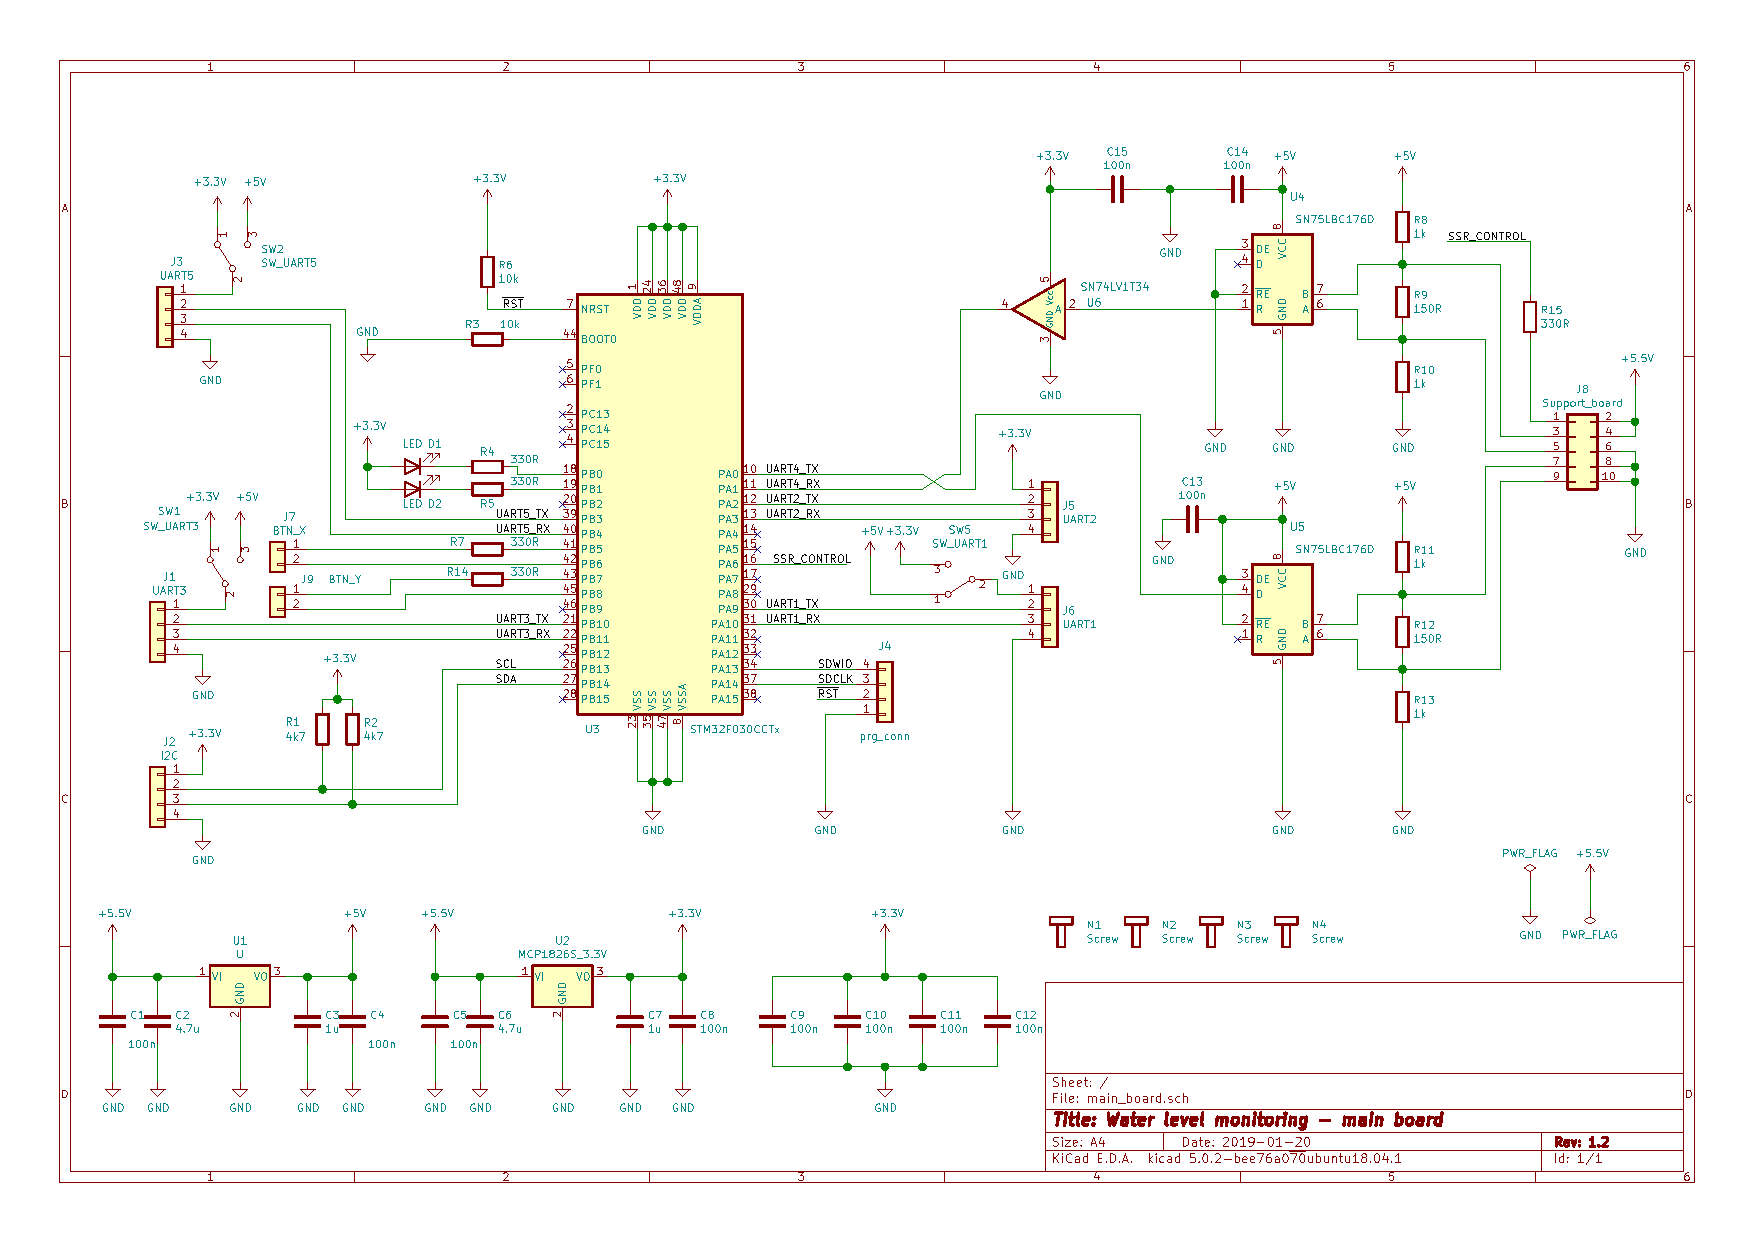
\includepdf[landscape=true, offset=20 -40]{obrazky-figures/main_board_scheme.pdf}

\chapter{Plošný spoj pro řídicí desku}
	\label{sec:main_board_pcb}
    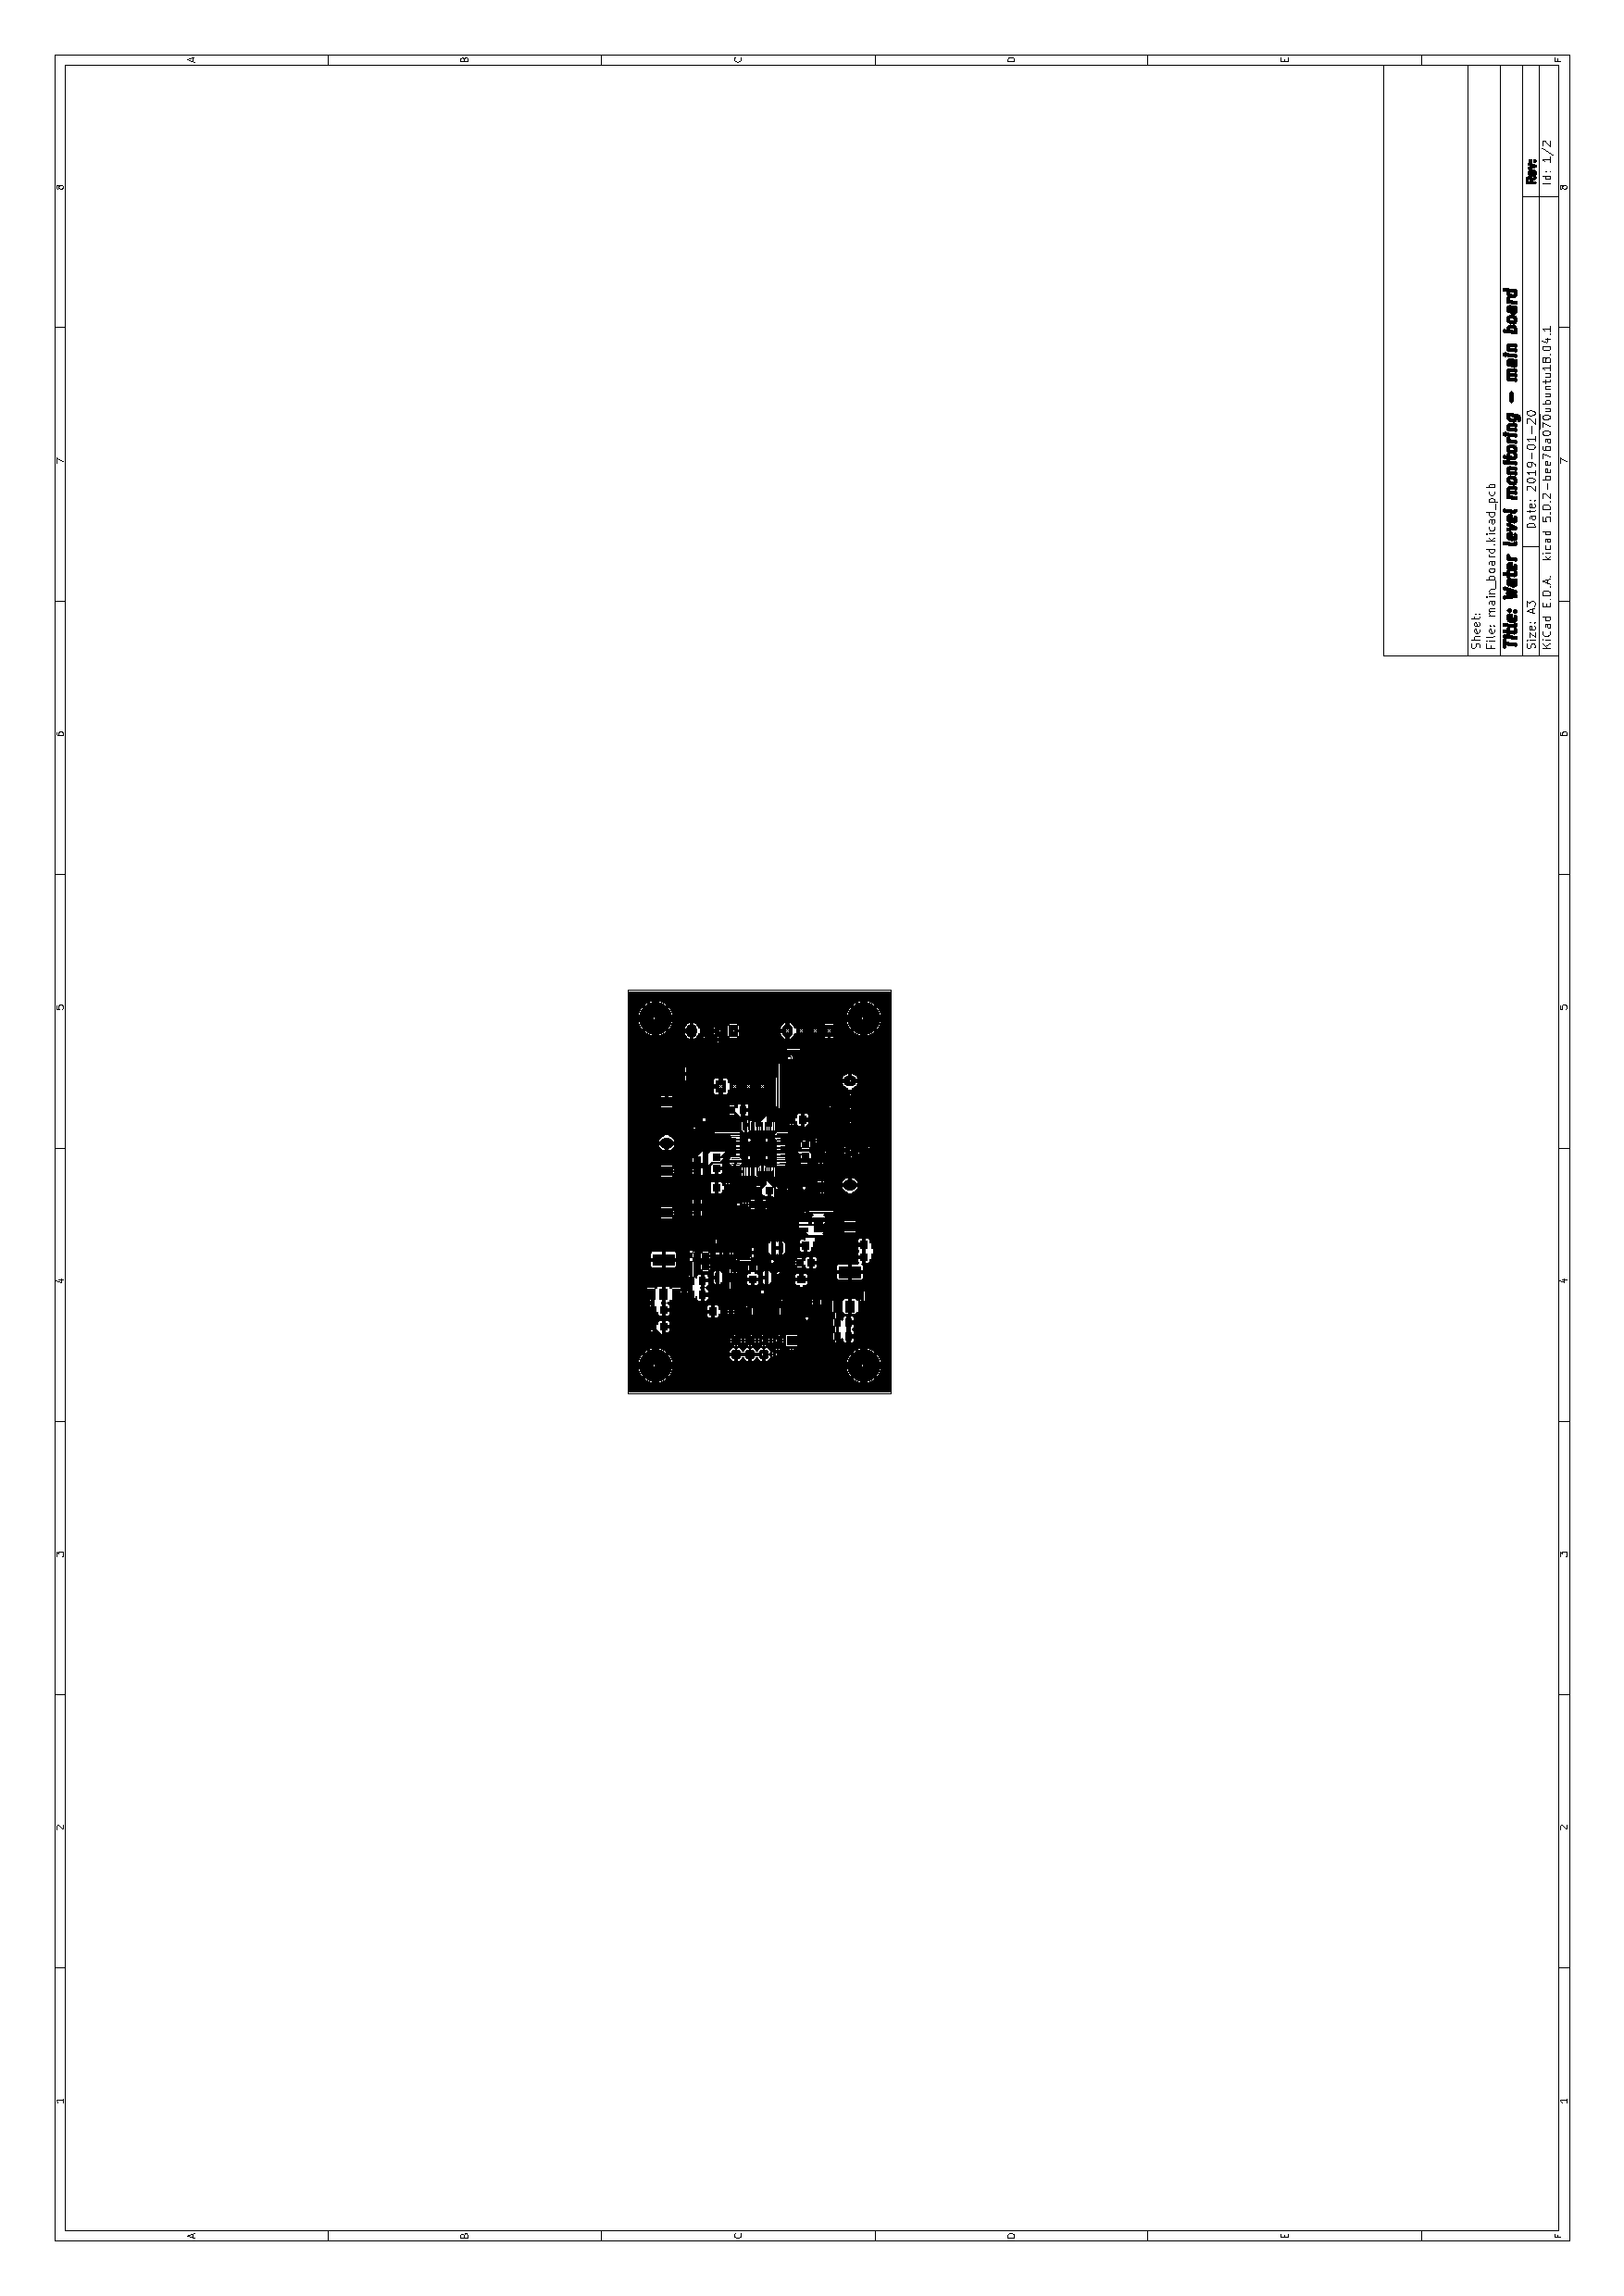
\includepdf[pages={1,2}, landscape=true, angle=270, offset=20 -40]{obrazky-figures/main_board_pcb.pdf}

\chapter{Schéma podpůrné desky}
	\label{sec:support_board_scheme}
	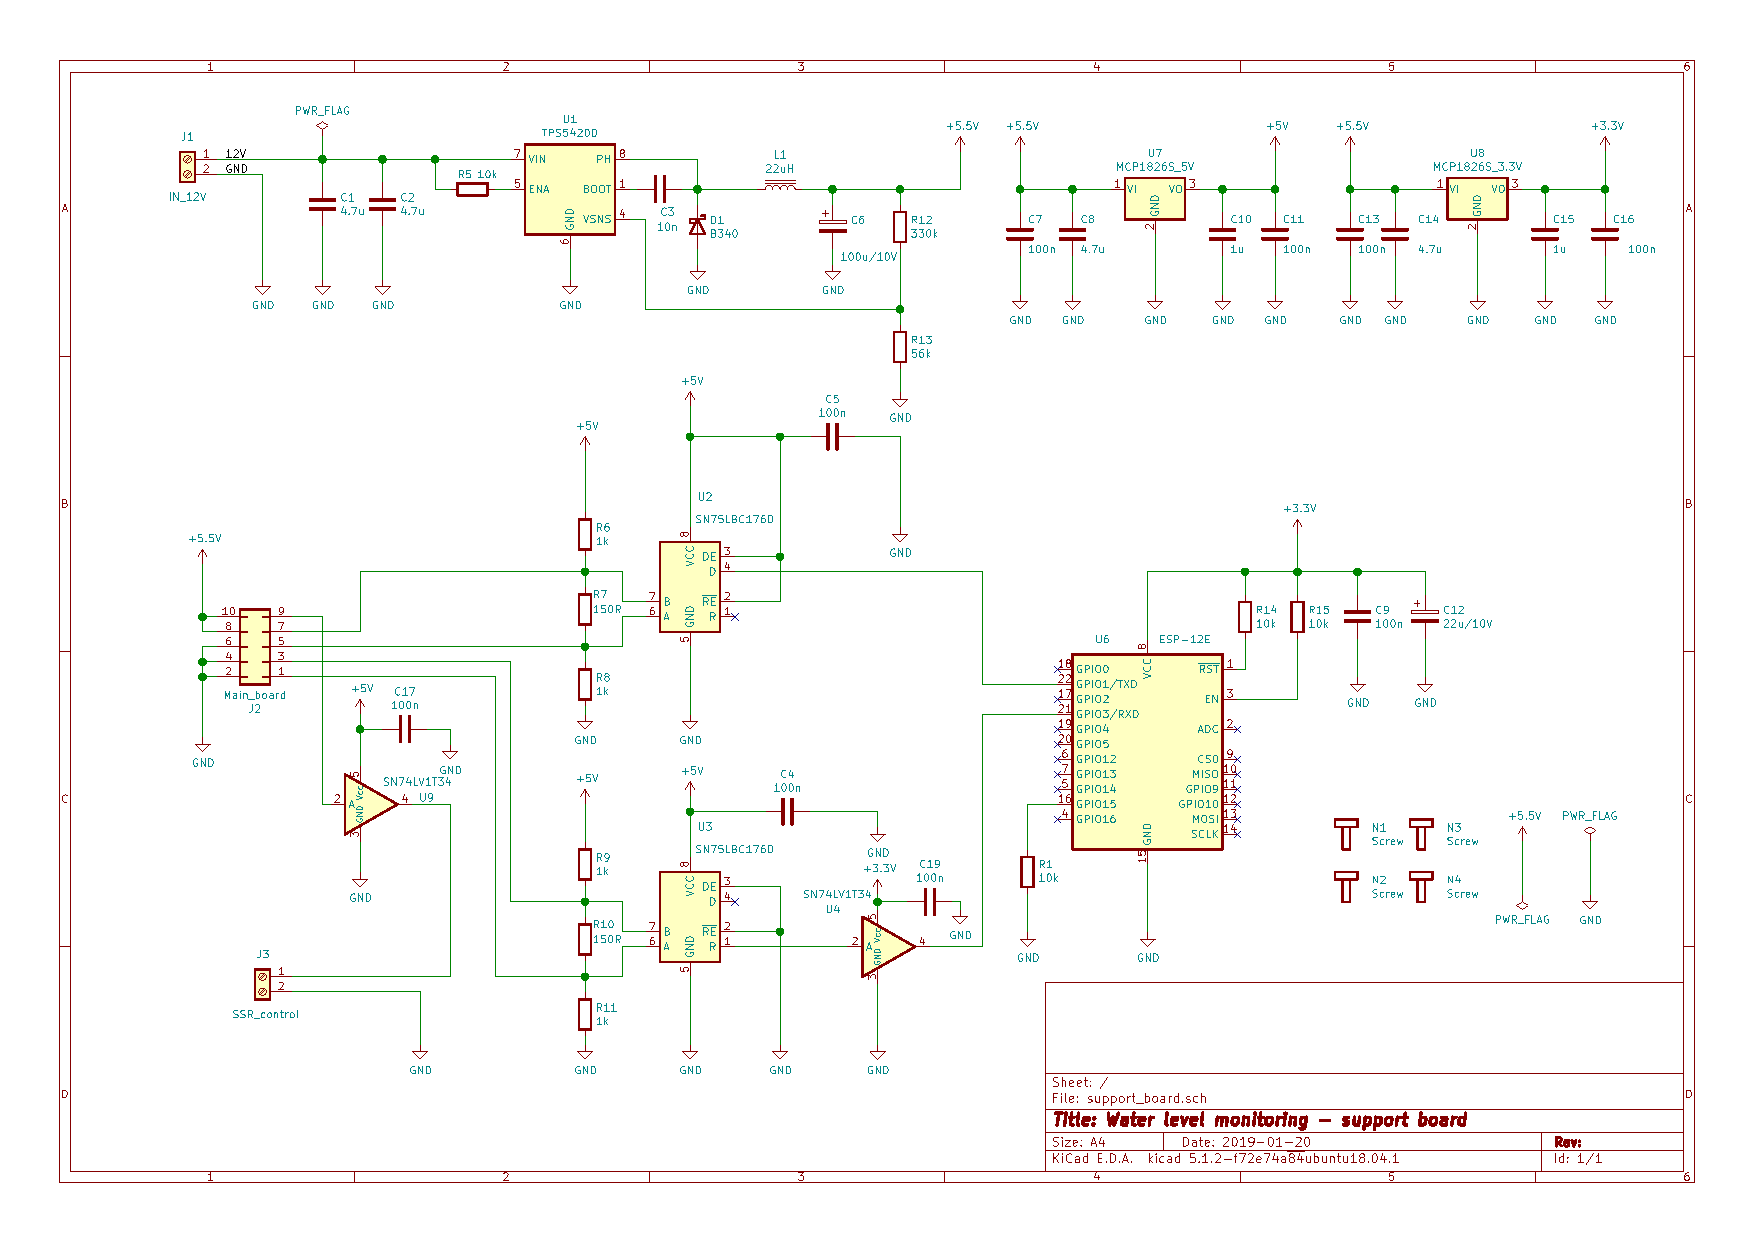
\includepdf[landscape=true, offset=20 -40]{obrazky-figures/support_board_scheme.pdf}

\chapter{Plošný spoj pro podpůrnou desku}
	\label{sec:support_board_pcb}
	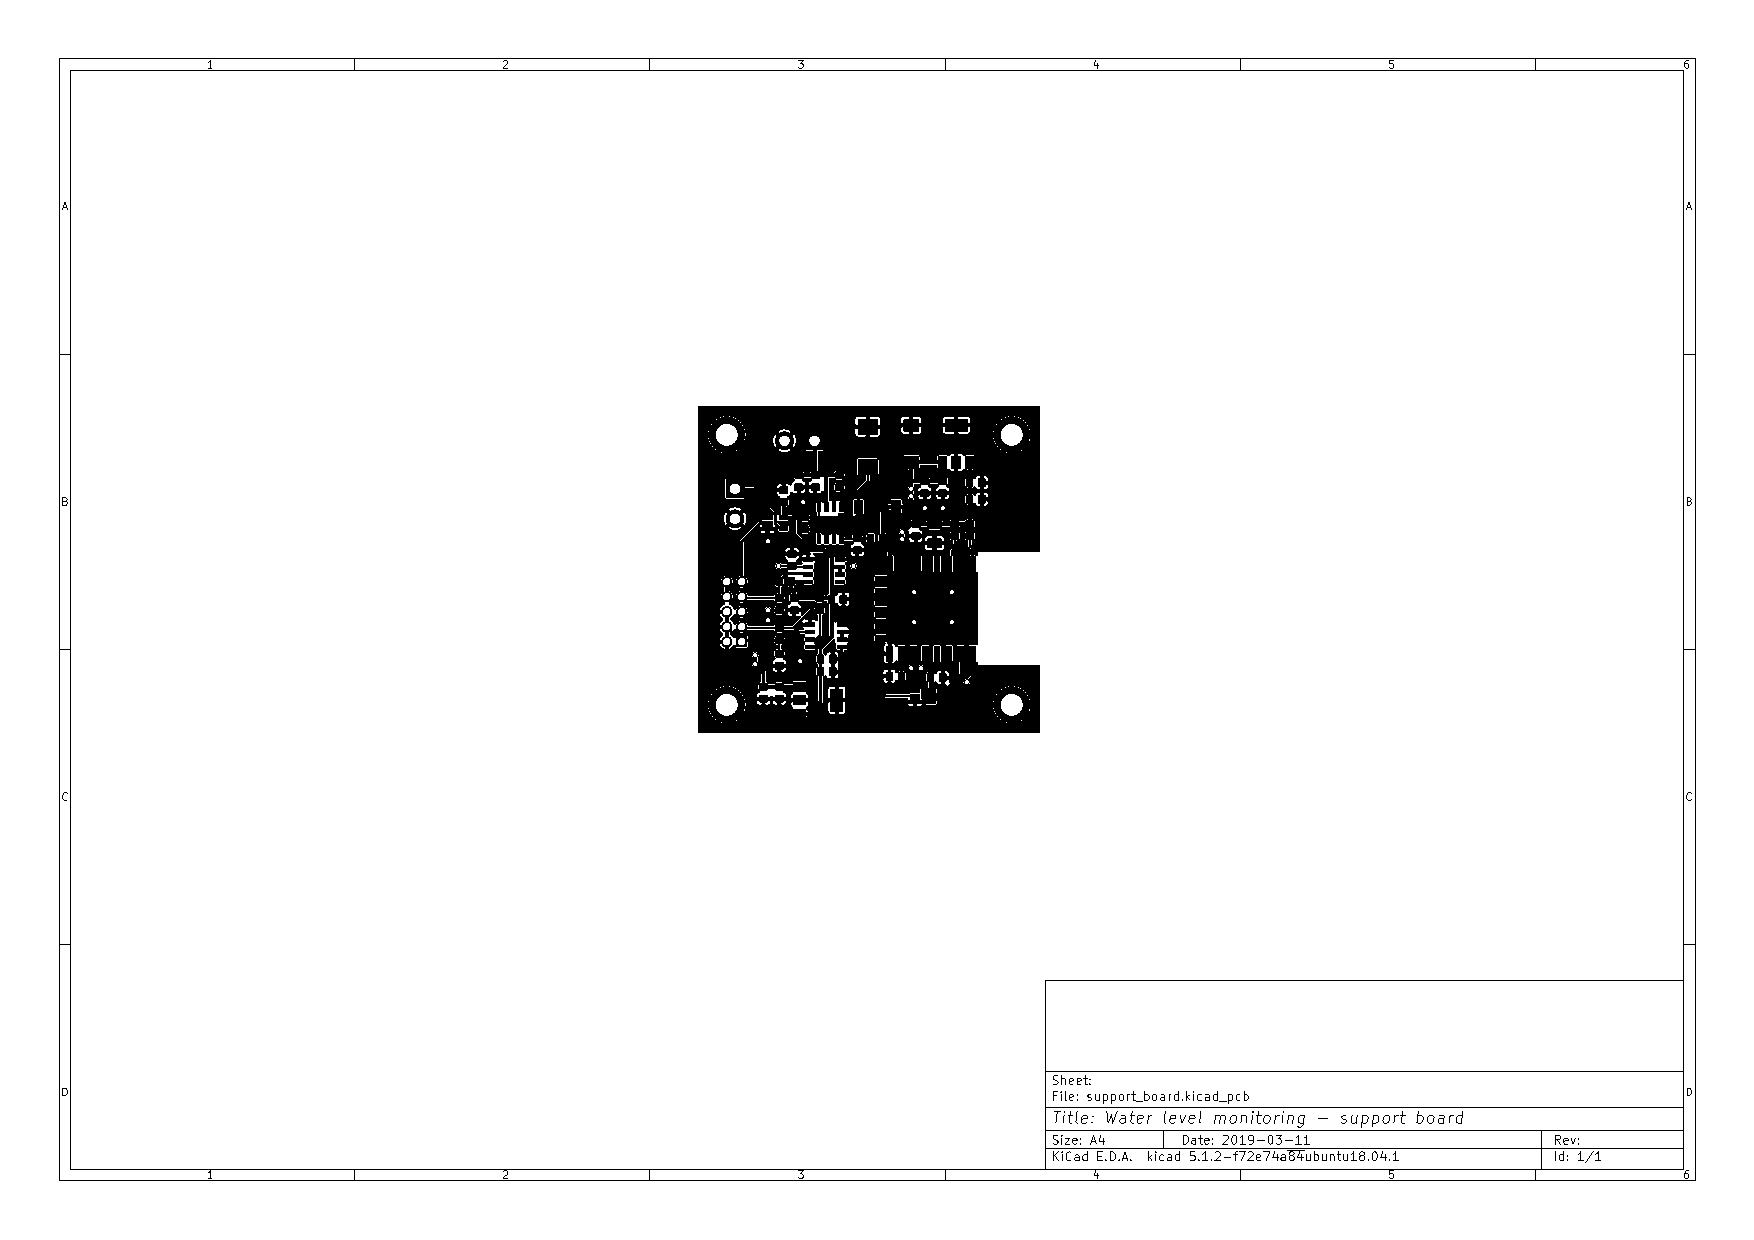
\includepdf[pages={1,2}, landscape=true, angle=270, offset=20 -40]{obrazky-figures/support_board_pcb.pdf}
